


\chapter{Implementation}
This chapter discussed the technical implementation of the system based on the design discussed before.
Section 4.1 provides the technical information about the main entity as classes that will be used in this study, including its variables and methods.
section 4.2  provides a complete information about the work flow of the application.
Section 4.3 provides an information about the mechanism of notification. Lastly, section 4.4 provides an information about the tracker and its procedure.

Flask framework and python programming language is used to develop the webserver. Java programming language and Android SDK is used to develop android application.

% \subsection{Web server}
% explain sending data to the android application
% Webserver is a http server that
% send a json file


%explain get data from android appplication


\section{Entities relationship}
All the entities discussed in the design chapter will be represented as a class which consists of variables and methods.
The relationship between classes can be seen on the class diagram on figure \ref{fig:class_diagram}.
 The box presents the class. The upper part of the box consists of the variable name and its type.
 The plus and minus sign before the variable name present the scope of the variable.
  Minus (-) means private and plus (+) means public.
  The bottom part of the box consists of the class methods and the type of its output.
  Furthermore, the arrow present the variable relationship whether it can be one-to-one (1..1)  or one-to-many(1..*) relationship.
  The arrow also present that a class extend other class which means it has same properties and methods.

\begin{sidewaysfigure}[ht]
\begin{center}
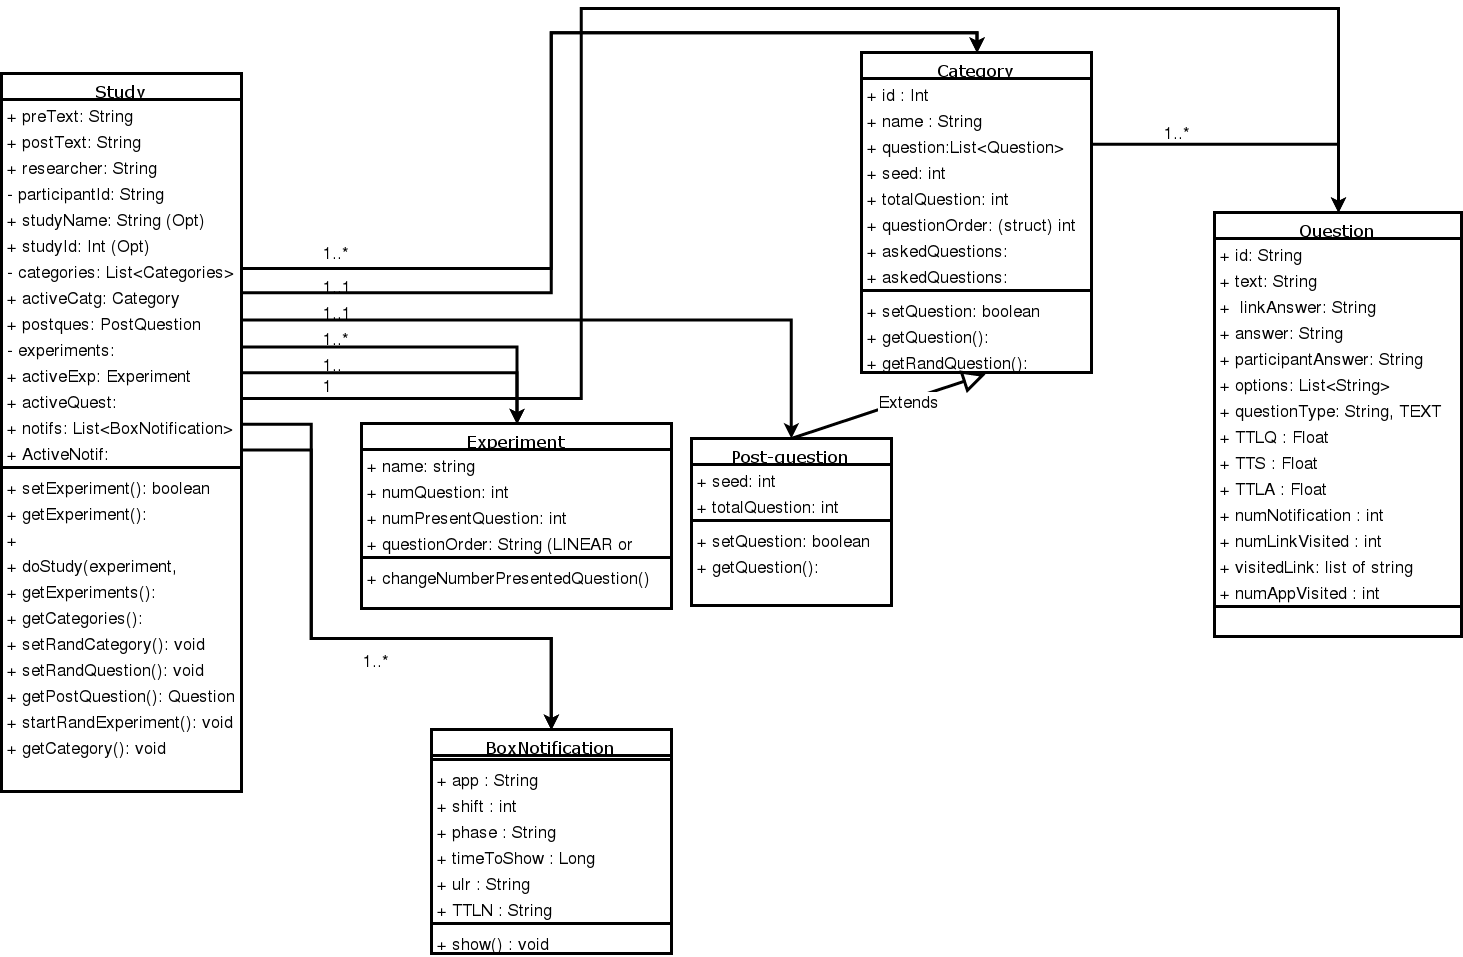
\includegraphics[scale=0.3]{class_diagram}
\end{center}
\caption{Class diagram of the application}
\label{fig:class_diagram}
\end{sidewaysfigure}

\subsection{Study Class}
Study class is the class that acts as a central container for other entities of the application, and it controls the flow of the main function of the experiment.
Some of its properties are defined from an input file; \textit{preText, postText, researcher, studyName, studyId}.
As seen in the class diagram \ref{fig:class_diagram}. The study class contains \textit{experiments} variable which consists of a list of experiment objects.
 \textit{Categories} variable which consists of a list of category objects, and \textit{notifs} variable that consists of a list of notification objects.

As explained in the design section, the experiment application need to initialize following variables before conducting the experiment;
\textit{ActiveExp} (active experiment) variable is experiment that will be conducted, and \textit{activeCatg} (active category) is the
category that will be used to pick questions.
\textit{ActiveQuest} (active question) variable present what questions are currently asked to the participant.
The question inside \textit{activeQuest} variable are picked from the a list of questions inside the active category (\textit{activeCatg}) variable.
\textit{ActiveExp} is set by the researcher on the setting experiment window, and the \textit{activeCatg} is chosen by the participant during the experiment



%After the category (\textit{activeCatg}) and set the experiment %(\textit{activeExp}) are chosen, the experiment can be started. The experiment will present the participant with one or several questions. In the study class there is \textit{activeQuest} (active question) variable that contains the  question objects that is being on a \textit{shift}.

Moreover, the class also contains \textit{activeNotif} (active notification) variable.
This variable contains a list of notifications that have been presented to the participant.
The notification object is picked from the \textit{notifications} variable that contains all the notification.

% \begin{table}[!b]
%   \centering
%   \begin{longtable}{ |p{0.5cm}|p{4cm}|p{2.3cm}|p{6cm}|  }
%  \hline
%  No& Variable's name & Type & Description \\
%  \hline
%  1 & preText & string  & the text\\
%  2 & postText & string & THIS DESCRIPTION NEED TO BE FILLED\\
%  3 & researcher & string & True if the participant decide to look at the question again, false otherwise. \\
%  4 & studyName & string & total time (in millisecond) when the participant see the answer links and decide to look the question again or answer the question (next button) \\
%  5 & studyId & string & Similar with TTLB and the participant decide to look at the question again.Then, answer links are shown again to the participant\\
%  6 & participantId & List of String & The list of links clicked/visited by the participant after clicking the answer links\\
%  7 & randomGenerator & List of Long  & List of the total time (in millisecond) the participant stay on a page after clicking link\\
%  8 & categories & List of String & similar with visited\_links but the participant have decided to see the question again then return to the answer links window\\
%  9 & experiments & List of Long & Similar with time\_visited\_links but the participant decide to look at the question again then click the answer links\\
%  10 & postques & Long & Total time (in millisecond) the participant see the fill answer window and then click next\\
%  11 & activeExp & Long & Total time (in milisecond) the participant write the answer on the text box\\
%  12 &  activeCatg & Integer & how many notification is shown during the a question \\
%  14 & activeQuest & Long & Total time (in millisecond) it tooks the participant after clicking the notification to back to experiment application\\
%  15 & notifs & Long & Total time (in millisecond) it tooks the participant after clicking the notification to back to experiment application\\
%  16 & activeNotif & Long & Total time (in millisecond) it tooks the participant after clicking the notification to back to experiment application\\
%  16 & shiftNum & Long & Total time (in millisecond) it tooks the participant after clicking the notification to back to experiment application\\

% \hline
% \end{longtable}
% \caption{Variable inside study class}
%  \label{tab:studyClassVariable}
% \end{table} \par
\subsection{Experiment Class}
The Experiment class contains the \textit{experiment variables} that is used to define the behavior of the experiment.
The variables are explained in the table \ref{tab:ExperimentClassVariable}.
Every variables inside this class except \textit{numPresentedQuestion} is determined from the input file. \textit{numPresentedQuestion} is a variable that
control how many questions is presented to the participant each time.
 \textbf{changeNumberPresentedQuestion()} method is called by the study class to change the value \textit{numPresentedQuestion} variable.
 The change can be random (from 1 to \textit{maxPresentedQuestion}) by using the Random object (RandomGenerator)
  provided by Java API.

\begin{table}[!htb]
  \centering
  \small
  \footnotesize
\begin{tabu}{|X[0.5,l]|X[5,l]   |X[2.3,l]|X[6,l]|  }
 \hline
 No & Variable's name & Type & Description \\
 \hline
 1 & name & string  & The name of the experiment\\ \hline
 2 & numQuestion & Integer & The number of questions will be asked on the experiment \\ \hline
 3 & numPresentedQuestion & Integer & The number of question presented to the participant on the experiment every phase of question-answer \\ \hline
 4 & questionOrder & String & If the value is RANDOM, then the question is picked randomly from a list of question, if the value is LINEAR then the question will be picked based on the order of the input file \\ \hline
 5 & randomPresentedQuestion & Boolean & If it the value is true, then on each phase the num of presented question will changed randomly, explained more on changeNumberPresentedQuestion method \\ \hline
 6 & maxPresentedQuestion & Integer & This is the maximum number of presented question if the number of presented question is decided randomly\\ \hline
 7 & randomGenerator & Random  & This is a random class that use to generate random nunmber, it is used inside changeNumberPresentedQuestion method \\ \hline
\end{tabu} \par
\caption{variables inside the experiment class}
 \label{tab:ExperimentClassVariable}
\end{table}

\subsection{Category Class}
Category class is used to carry the questions objects.
It has two main variables; \textit{questions} and \textit{askedQuestion}.
\textit{Questions} variable consist a list of questions. This variable is filled by
the question from the input file.
\textit{AskedQuestion} variable consists of all the question that had been asked.

The class has two main methods \textit{getRandQuestion()} and \textit{getQuestion()}.
These methods will be called during the quiz activity to put question object into activeQuestion variable.
These methods are two different procedure to pick a question from \textit{questions} variable.
the former takes the question randomly while the latter takes the question based on the order of the input file.
Java random class is used to generate random index (from 0 to the size of the \textit{questions} variable).
After the question is selected, it will get deleted from the \textit{questions} variable and then it will be put it into \textit{askedQuestion} variable.

\subsection{Question Class}
Table \ref{tab:questionClassVariable} shows the variables inside this class.
The \textit{question} class consist of the content of question; its question text, answer link and answer.
The class also contains the tracked variable (the variables are explained more on trackker section).
The question can be two type MC or TEXT. MC means multiple choice, this question type will have multiple options on its answer choice,
and the participant can chose one of them. while TEXT means that the participant need to write the question.
\textit{representId} is generated when the questions are presented to the participant. this variable is unique and can
be used to classify which questions are presented at the same time.

\begin{table}[!tbh]
  \centering
  \small
  \footnotesize
  \begin{tabu}{|X[0.5,l]|X[4,l]|X[2.3,l]|X[6,l] |}
 \hline
 No & Variable's name & Type & Description \\
 \hline
 1 & id & string  & The id of the question.\\  \hline
 2 & text & string & The text of the question.\\ \hline
 3 & linkAnswer & string & the URL link to the answer page. \\ \hline
 4 & answer & string & (optional) the answer of the question. \\ \hline
 5 & participantAnswer & string & the answer of the participant during the quiz activity.\\ \hline
 6 & questionType & String & The type of the question. The value can be "MC" or "TEXT".\\ \hline
 7 & representId & string  &  the random id generated when the question is presented during quiz.\\ \hline
 7 & options & list of String  & The answer option if the question is multiple choice.\\ \hline
\end{tabu}
\caption{Variable inside Question class (without the tracked variable)}
 \label{tab:questionClassVariable}
\end{table} \par

\subsection{BoxNotification class}
BoxNotification is used as a class name because the name Notification is already defined inside the Android framework.
Most of the variable in this class is similar to the defined variable in the design section.
Similar to the question class, the notification also contains \textit{presentedID} which show
on which question the notification is shown.
The content of the notification can be set into \textit{title} and \textit{msgText} variable.
The Notification can open an android application of twitter, facebook, instagram and web browser. The application should be installed on the phone, otherwise, the notification will open the url of the application on the web browser.
To define which user will be shown if the user clicked the instagram, twitter or facebook notification. The user
is defined by the user\_id code which can be found on the profile of their social media.
the url can also contain the URL link, then the application will open the web page.
This app needs to be specified on the \textit{app} variable and the \textit{url} variable. The \textit{url} variable needs to be filled with the user id of the twitter or instagram. Or it can be filled with http/https url to open web page. the class contains a show() method that will pop up the notification in the android phone.
The mechanism and flow of the notification will be explained on next chapter.

%
% \begin{table}
%   \centering
%   \small
%   \footnotesize
% \begin{tabu}{ |X[0.5,l]|X[4,l]|X[2.3,l]|X[6,l]|  }
%  \hline
%  No& Variable's name & Type & Description \\
%  \hline
%  1 & url & String & this contains  \ \hline
%  2 & titleText & Integer & this is the maximum number of presented question if the number of presented question is decided randomly\\ \hline
%  3 & msgText & Random  & this is a random class that use to generate random nunmber, it is used inside changeNumberPresentedQuestion method \\ \hline
%  4 & presentedID & Random  & this is a random class that use to generate random nunmber, it is used inside changeNumberPresentedQuestion method\\
% \hline
% \end{tabu}
% \caption{variable inside notification class, some of the variable are already discussed on the design section}
%  \label{tab:NotificationVariable}
% \end{table}

\section{Application flow}
In this section, the flow of the application from the technical point of view is provided.
The flow of the application can be seen
on figure \ref{fig:flowOfApplication}. The figure shows the flow of the application after input file is uploaded and
the experiment just has started.
As it seen in figure, the flow is divided into four scopes;
\begin{itemize}
\item \textbf{Setting}  : the researcher can set some properties of the experiment or choose to start the experiment.
\item \textbf{Experiment} : The participant conducts the quiz experiment.
\item \textbf{Notification} : The notification can be shown during the quiz.
\item \textbf{PostQuestion} : The participant presented with post questions.
\end{itemize}
\par

To have further understanding about the application flow, the activities and method on the flow chart is explained further in the following subsection.



\begin{figure}
\begin{center}
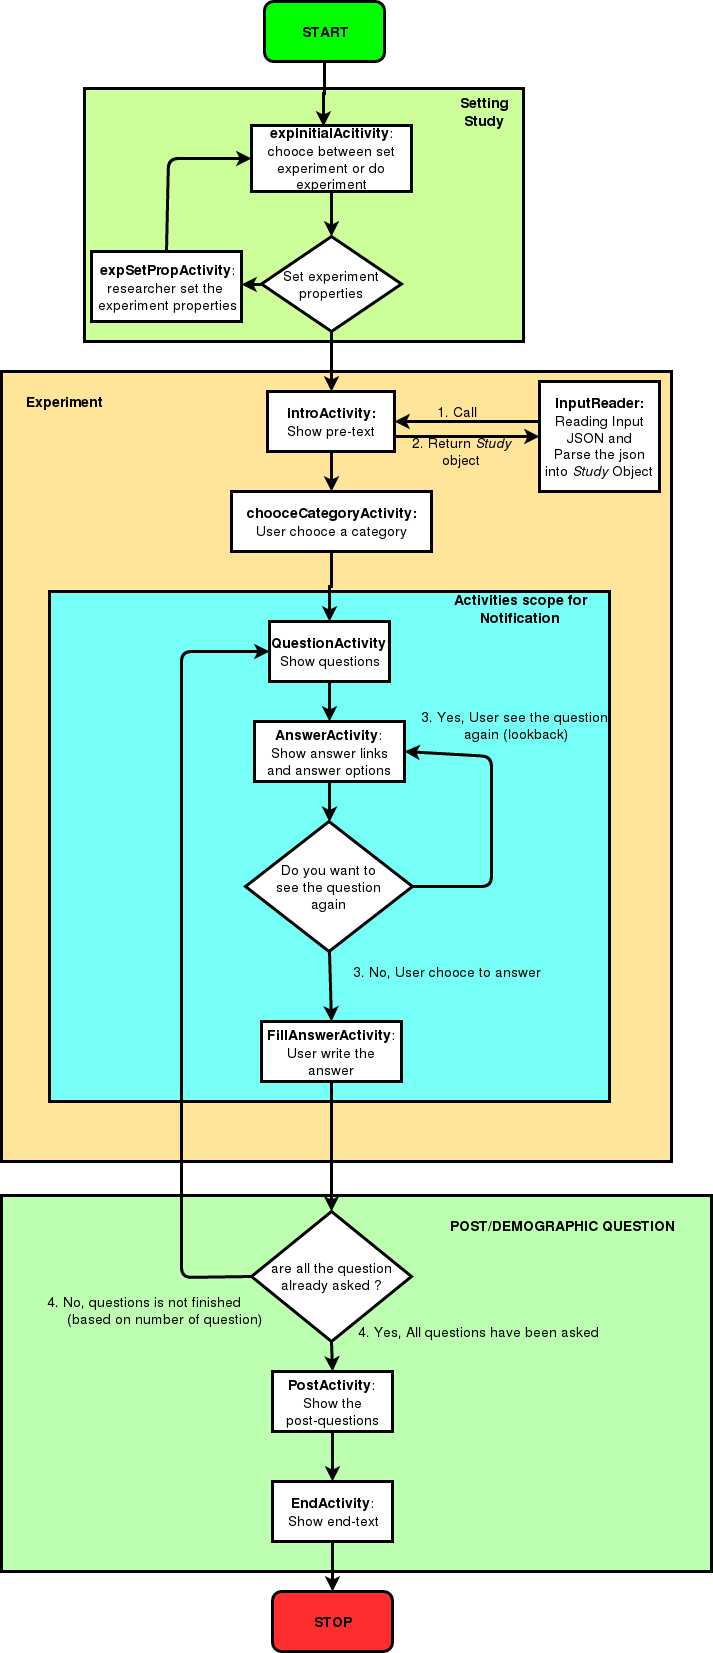
\includegraphics[scale=0.4]{Flowchart_}
\end{center}
\centering
\captionsetup{justification=centering}
\caption{The flow of the application}
\label{fig:flowOfApplication}
\end{figure}

\subsection{Android Activity}
The android application built upon multiple class activities.
Each activity has a user Interface (UI) template. this template is saved into an xml file. The template consist of UI element, for example, button, text, etc.
Its corresponding class activity will decide what will appear on the phone or what happens if a button is clicked.
For example answerActivity class will have activity\_answer.xml template.
The activity class is used to catch the event such us clicked or move to another application. This event is linked to an \textit{event listener} methods.

The android application also contains a lifecycle which is  default methods and activities that will be called everytime.
Figure \ref{fig:theLifeCycleOfActivity} shows the android activity lifecycle \citep{androidActivity}.
There are three methods inside the lifecycle that is used in this experiment application;
 \textit{OnCreate()} is the first method to get called everytime the activity start.
 \textit{OnPause()} will be called if the phone move to another application.
 Lastly,  \textit{OnResume()} is called if the user open the application again after leave the application.

\begin{figure}[!tbh]
\begin{center}
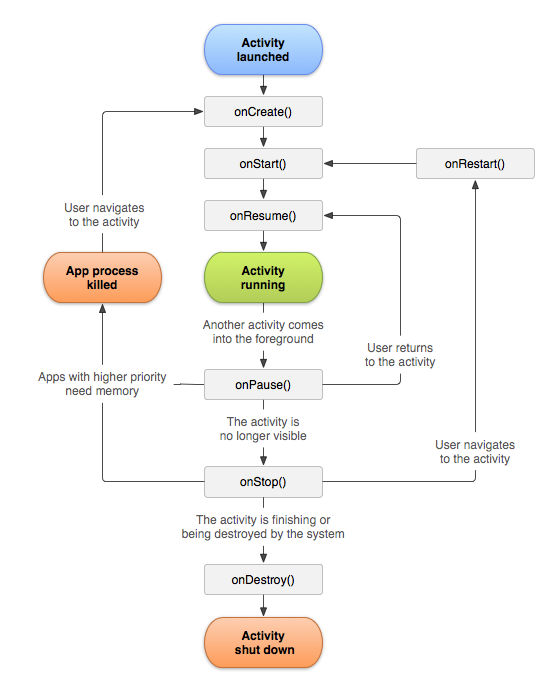
\includegraphics[scale=0.5]{activityLifeCycle}
\end{center}
\centering
\captionsetup{justification=centering}
\caption{The lifecycle of android application}
\label{fig:theLifeCycleOfActivity}
\end{figure}



\subsection{expInitialActivity}
The UI layout of this activity can be seen in figure \ref{fig:expInitialActivity}.
The participant can click a button to begin the experiment or to set the properties of the experiment.
On the \textbf{OnCreate()} method the \textbf{InputReader.read()} method is called firstly.
This method will read the JSON input and compiled it into \textit{Study} object.
String input is compiled into json object by using \textit{GSON} library.
\textit{GSON} is a serialization / deserialization library that is used to convert a string into a json object or another way around. \citep{gsonLib}

Then the json object compiled into The \textit{Study} object. This object controlled the quiz experiment and hold all the data, including the track variables.
This object will be sent through the activities.
\textit{Intent} class of java is used to encapsulate the object and send to another activity.
Because the \textit{Study} object need to be encapsulated inside the Intent,
 java programming language require every class including the Study class to implement \textit{Serializable}.

%
% \begin{figure*}
% \centering
% \begin{minipage}[b]{.4\textwidth}
% 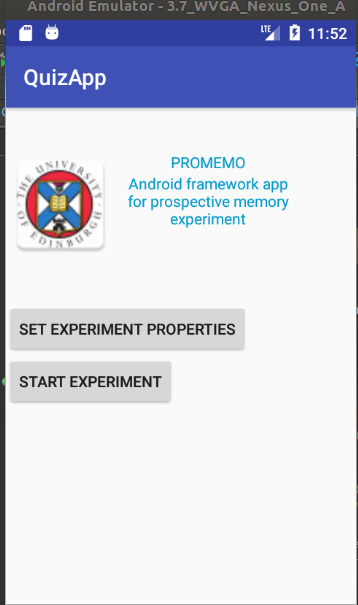
\includegraphics[scale=0.32]{FE_1}
% \caption{Caption}\label{label-a}
% \end{minipage}\qquad
% \begin{minipage}[b]{.4\textwidth}
% 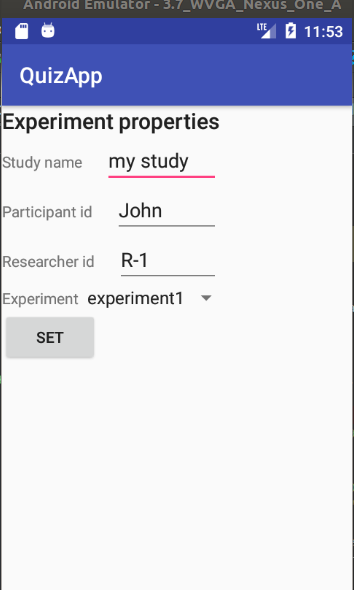
\includegraphics[scale=0.32]{FE_set_properties}
% \caption{Caption}\label{label-b}
% \end{minipage}
% \end{figure*}

\subsection{expSetPropActivity}
The UI layout of this activity can be seen in figure \ref{fig:expSetPropActivity}.
This activity is used to set some parameter of the experiment. In this activity the researcher can pick which experiment to conduct, the name of the experiment,
the id of the researcher and the id of the participant.
The purpose of this activity is to make it easier for the researcher to conduct multiple experiments and multiple participants without uploading the input file again.

\subsection{IntroActivity}
The UI layout of this activity can be seen in figure \ref{fig:IntroActivity}.
This activity is used to show the information about the experiment to the participant before starting the experiment.
This information is obtained from the preText and postText variables. the value of this variable will be converted into a html and shown to the participant.
Figure X show example of the Consent information shown inside the application.

\subsection{ChooseCategoryActivity}
The UI layout of this activity can be seen in figure \ref{fig:ChooseCategoryActivity}.
In this activity the participant chooses which category he/she want to answer.
The selected category name will then save in the \textit{selectedCategoryName} variable inside study class.
\textit{selectedCategoryName} is used to in the experiment initialization to initialize \textit{activeCatg} variable


\subsection{QuestionActivity}
The UI layout of this activity can be seen in figure \ref{fig:QuestionActivity}.
In this activity, the question inside \textit{activeQuestion} variables is shown to the participant.
This activity will be called multiple time during the quiz experiment.
the main function of this activity is to call \textbf{Study.runExperiment()} method.
\textbf{Study.runExperiment()} is used to start or continue the quiz experiment.
this method is explained in the section below.

\subsubsection{Study.RunExperiment()}
This method will be called everytime the Quiz activity started.
The main function of this methods are :
\begin{itemize}
\item Initialize the active experiment (\textit{activeExp} variable) and active category (\textit{activeCatg}) variable.
\item Change the number of \textit{presentedQuestion} (the variable is explained in the Experiment class section).
\item Set the active questions (\textit{activeQuest}) from the questions in the category.
\end{itemize}


\begin{figure}
\begin{center}
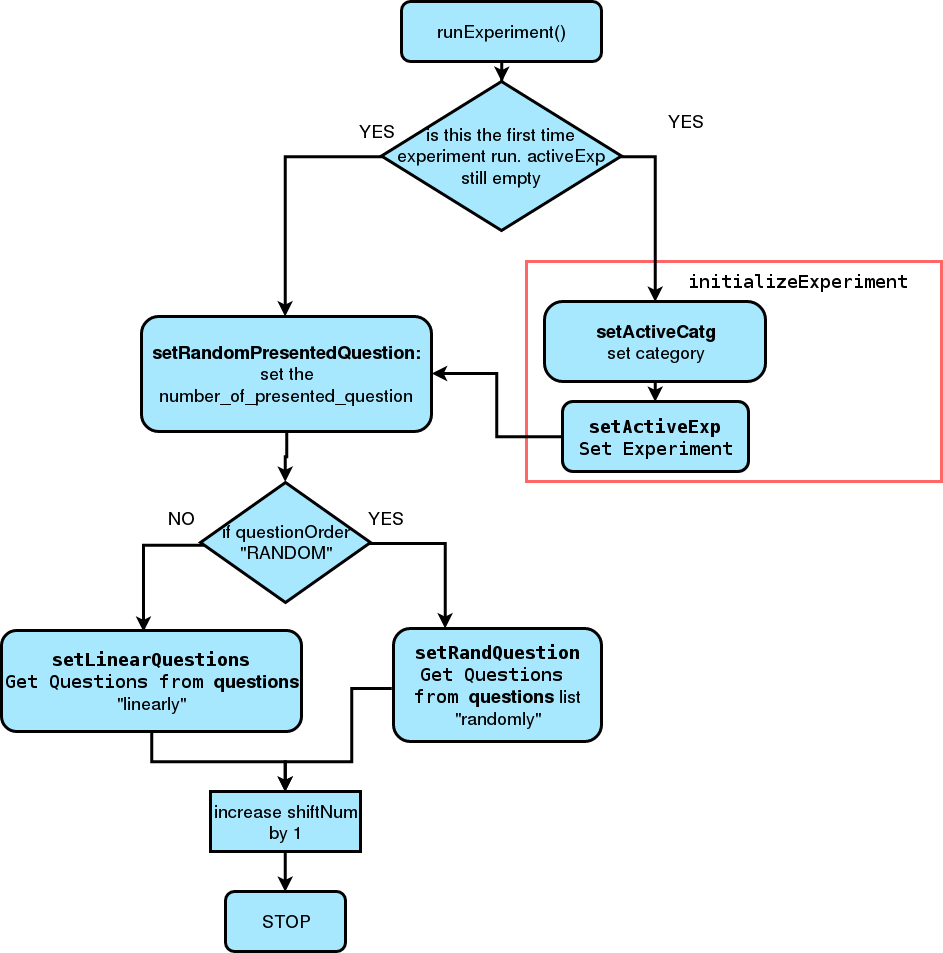
\includegraphics[scale=0.45]{runExperiment}
\end{center}
\caption{Flow chart of runExperiment method}
\label{fig:runExperiment_flow}
\end{figure}


Figure \ref{fig:runExperiment_flow} shows the work flow of the method. The First step is to initialize the experiment by checking the active experiment (\textit{activeExp}) variable.
 if it's empty then it's the begining of the experiment, hence some variables needs be initialized. If it's mean that the experiment had been started (on-going)
 so new question is presented to the participant.


On the inisialization, active experiment (\textit{activeExp}) and active category (\textit{activeCatg}) are initialized by calling \textbf{initializeExperiment} method.
The \textbf{initializeExperiment} method will fetch the selected \textit{experiment} and the
\textit{category} object from the study class variables based on the \textit{selectedExperimentName} and \textit{selectedCategoryName}.


Subsequently, the \textbf{setRandomPresentedQuestion()} is called, this method will set the value of \textit{numPresentedQuestion}.
If the researcher set randomPresentedQuestion to true in the input file, then \textbf{Experiment.changeNumberPresentedQuestion()} is called, this method will set numPresentedQuestion randomly
On the other hand if it's false, then the numPresentedQuestion will be constant.

Next, \textbf{isExperimentIsStillGoing()} is called. This method make sure if the experiment is still on progress by checking the size of the
\textit{question} variable inside the \textit{activeCatg}. If the size is still larger or similar then \textit{numPresentedQuestion} then the experiment can be continued.

Lastly, the active question (\textit{activeQuest}) is picked from the questions variable by calling \textbf{setActiveQuestion()}. this method filled
 i \textit{activeQuest} variable by fetching \textit{question} object from the \textit{question} variable inside \textit{activeCatg} object.
  The question object will be picked randomly if the researcher set \textit{questionOrder} to random. Otherwise, it will be picked linearly based on
  the input file order.


\subsubsection{AnswerActivity}
The UI layout of this activity can be seen in figure \ref{fig:AnswerActivity}.
In this activity the answer link are shown as a textview inside the UI layout. If the participant clicks the answer
link then the \textbf{clickListener()} method inside the textview will open the answer page.
A java class called \textit{webview} is used as a browser. The \textit{webview} will open the web page based on the URL of the answer link (\textit{question.url}).

On the layout, two radio buttons are presented to the participant. These are the option whether the participant wants to return to see the question again or to continue
 to answer the question.
If the participant chose to look at the question again then a special string is capsulated inside the \textit{intent} object.
This string is sent to question activity then send back to answer activity. this string is used to indicate if the participant lookshidded at the question again.
If the string is sent to answerActivity then the radio button "to see the question again" is hidden.


\subsection{fillAnswerActivity}
The UI layout of this activity can be seen in figure \ref{fig:fillAnswerActivity}.
In this activity the participant should answer the question by writing the answer on the editText UI.
If the participant clicks next button then \textbf{saveAnswer()} method is called. this method will get the value of the editText
and stored it on the \textit{participantAnswer} variable inside the \textit{question} object.


\section{Notification mechanism}
Figure \ref{fig:NotificationFlo} shows the mechanism of notification.
As seen on the flowchart, the \textbf{checkNotification()} method is called inside
the OnCreate event on the QuestionActivity, AnswerActivity and FillAnswerActivity.
The method checks on every notifications inside the \textit{notifs} variable if the there is a notification that should be shown up based on \textit{phase} and \textit{shift} variable of the notification.

If there  is a notification that needs to be shown up then the notification object is added into the \textit{activeNotif} and it is deleted from the \textit{notifs} variable of the study object.

The notification needs to wait for some millisecond before it can be shown up. The waiting time is defined in \textit{timeToshow} variable inside the BoxNotification class.
While the notification process waits, the main activity should keep working, so another process needs to be spawned a part of the main process.
To accomplish it, \textit{TimerService} class is used. This class will be spawn as new process and it will sleep for \textit{timeToShow} millisecond.
After that, the service class will call the \textbf{BroadcastReceiver()}.
The \textbf{BroadcastReceiver()} method  is defined on all of activities, and it simply calls \textbf{show()} method of the notification.
The \textbf{Notifaction.show()} method is used to show  the notification to the front end of the android screen. This method use
 \textit{NotificationCompact.Builder} to build the notification layout.
 an \textit{Intent} object is inserted inside the Builder object that contains what application to open.
 If the participant clicks the notification then the experiment application will be minimized.
 This event will call \textbf{OnPause()} method on the current activity, and the android phone will open the intended application.
 The participant if the open the experiment application again, then the \textbf{OnResume()} method is called.


\section{Tracker}

The tracked variable are shown on the table \ref{tab:trackedVarible}.
All of these variable are stored inside the \textit{question} class as seen in the class diagram \ref{fig:class_diagram}.
Some of the variables are used to track the time in millisecond.
To track the time the \textit{stopWatch} class provided by java API is used.
The StopWatch object is stored inside the study class because the StopWatch class is not serizable.
During the experiment the application is minimized (participant clicks the notification).
Then event some Stopwatch object need to be paused. Inside \textbf{OnPause()} event listener the stopWatch is suspended,
and it will resume again inside the \textbf{OnResume()} event listener.

As seen in the class diagram, each one of tracked variable has its own \textit{stopWatch} object, for example \textit{stopWatchTTLQ} will track the time for TTLQ variable.
To get the millisecond time of the stopwatch a \textbf{StopWatch.getTime()} method is called.
Then to stored the tracked time, the \textbf{study.log()} method is called.
This method pass two arguments; what variable to track and which stopwatch object is used to track it.
for instance \textbf{study.log("TTLQ",stopWatchTTLQ)} will track the \textit{TTLQ} variable and use \textit{stopWatchTTLQ} to track the time.
All of the tracked variable is then stored to the \textit{question} object inside the \textit{ActiveQuest} variable.
How each variable is tracked is explained further on the subsection below.
The expalanation of the variables are explained on table \ref{tab:trackedVarible}.

\subsubsection{TTLQ, lb\_TTLQ and lookback}
These variables is tracked inside the \textit{questionActivity}.
\textit{StopWatchTTLQ} and \textit{stopWatchTTLQ\_lb} are used to track the time of this variable.
The stopwatch object starts to count the time when \textbf{OnCreate()} method is called.
The \textbf{Study.log()} method will be called to track the variable when the next button is clicked then the stopwatch is stopped.
The lookback variable will have true value if the participant chose to see the question again.

\subsection{TTLB and lb\_TTLB}
These variable are tracked inside the \textit{AnswerActivity}. Similar with TTLQ,
\textit{stopwatchTTLB} and \textit{stopWatchTTLB\_lb} are used to track these variable.
The stopwatch will start on \textbf{Oncreate()} method and it will be tracked when the participant clicks the next button.

\subsection{visitedLinks, timeVisitedLink}
These variable is tracked inside the \textit{AnswerActivity}.
\textit{StopWatchLink} then will be started, and it are used to track the time participant have spent on each web page inside the \textit{webview}.
The mechanism of the tracking is shown in figure \ref{fig:webViewTrack}. Firstly, the prevUrl variable is initialized,
this variable stored the previous link the \textit{webview} had opened. This \textit{webview} class has an event listener called \textbf{onPageFinished()}
 which will be called every time the web page has been finish loaded, for example when the participant clicks new  link and open new web page.
  Every time \textbf{onPageFinished()} is called and when the participant clicks the next button then \textit{updateVisitedLinks()} method is called.
  \textbf{updateVisitedLinks()} method then store the value of \textit{prevUrl}
 to visitedLinks variable and how long the participant spent on the web page to \textit{timeVisitedLinks}.

\subsection{TTLA and TTLFA}
These variable are tracked on the \textbf{fillAnswerActivty}. \textit{TTLA} is tracked using \textit{StopWatchTTLA}, while
\textit{TTLFA} is tracked differently because if there is more than one question then there will be multiple \textit{editText} for the answer field, and
each one of them need to be tracked.

\textit{stopWatchTTLFA} is made as a hashmap where the key is the id of the \textit{editText} element.
The id is made from the index of the \textit{question} inside the \textit{activeQuest} variable.
The value of the \textit{stopWatchTTLFA} is the stopwatch object correspond of each question and \textit{editText}.
On each \textit{editText} element, the event listener called \textbf{OnFocusChangeListener()} is attached to it. This event listener will be called if there is a
change of focus on the UI layout of the activity, for example if the user click an editText then click another editText. The event listener
 method get the id of which editText was active before. The id then stored inside the \textit{activeViewId} variable.
By using \textit{activeViewId} variable a stopwatch corresponding to the id will be picked from the hashmap.


\subsection{numNotif, numNotifClicked and TTLN}
As seen in figure \ref{fig:NotificationFlo}. The QuestionActivity, AnswerActivity and fillAnswerActivity  call \textbf{checkNotifaction()} method
which will find the notification that should be shown up to the screen. If the notification is found than the activity call the \textbf{inceraseNumNotif()} method.
This method will increase the \textit{numNotif} variable by 1.

If the notificiation is clicked then the \textbf{inceraseNumNotifisClicked()} method will be called inside the \textbf{broadCastReceiver} method on the current activity class.
This method will increase the number of \textit{numNotifClicked} variable by 1.

\textit{NotifStopWatch} object is used to track the TTLN time.
After the participant clicks the notification than the application will be minimized and other
application will be opened.
 the \textbf{OnPause()} event handler will be called just before the application is minimized.
then inside the event handle a \textbf{Study.startLogNotif()} method is called. The \textbf{Study.startLogNotif()}  method will start the notifStopWatch object.
Then after the participant return to the experiment application the \textbf{onResume()} method is called.
This method will call \textbf{Study.stopLogNotif()} method.
The \textbf{Study.stopLogNotif()} method then track the TTLN variable inside the active notification
by using the \textit{notifStopWatch} object.

%\todo[inline]{WHAT THE FUCK TO WRITE}

\begin{sidewaysfigure}[ht]
\begin{center}
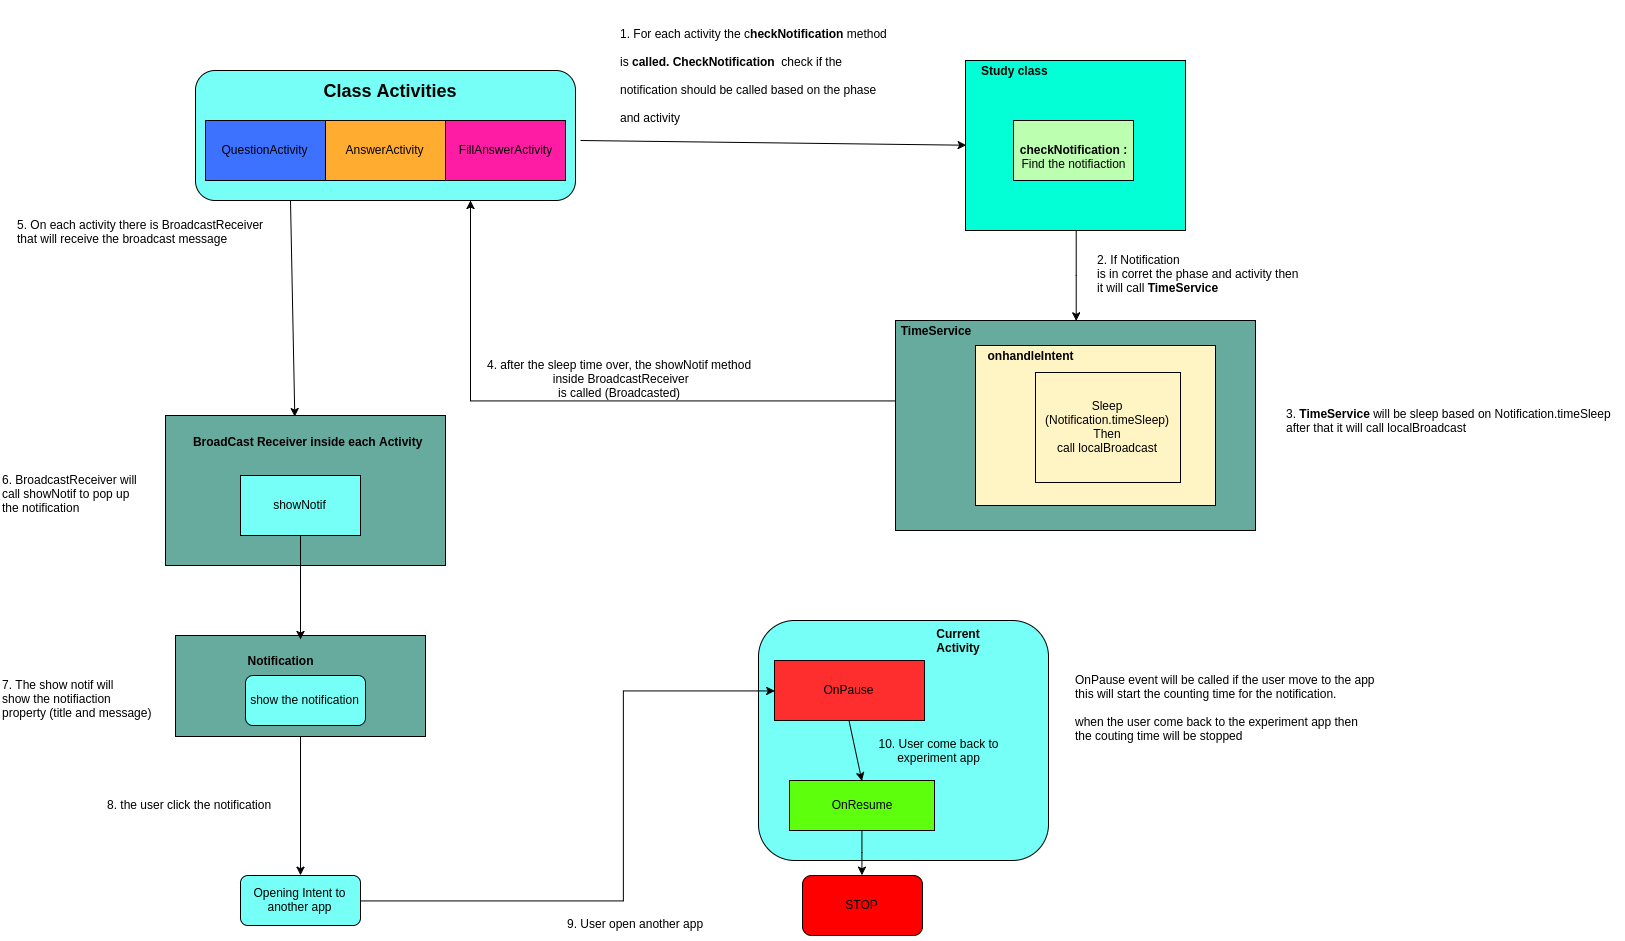
\includegraphics[scale=0.35]{notification_diagram}
\end{center}
\caption{The flow of the notification}
\label{fig:NotificationFlo}
\end{sidewaysfigure}
%
\begin{figure}
\begin{center}
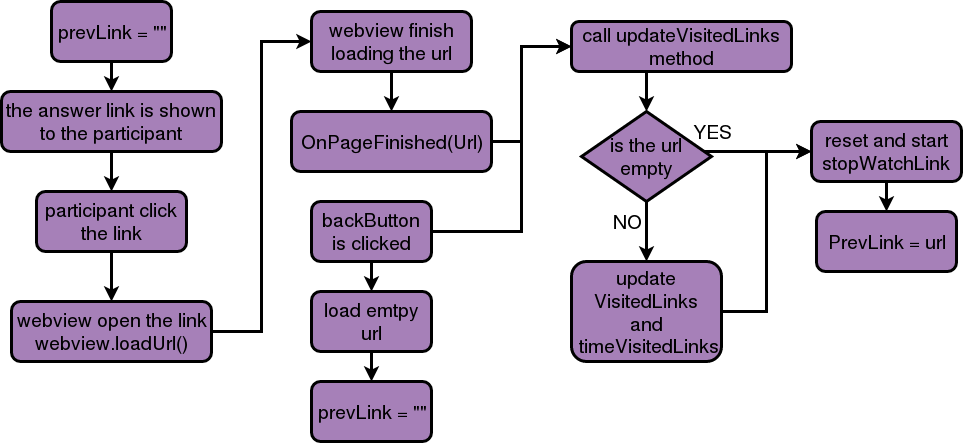
\includegraphics[scale=0.45]{tracker_linkVisited}
\end{center}
\caption{tracker mechanism for webview}
\label{fig:webViewTrack}
\end{figure}
